% !TEX encoding = UTF-8 Unicode
\documentclass[a4paper]{article}

\usepackage{color}
\usepackage{url}
\usepackage[T2A]{fontenc} % enable Cyrillic fonts
\usepackage[utf8]{inputenc} % make weird characters work
\usepackage{graphicx}
\usepackage{float}
\usepackage[english,serbian]{babel}
%\usepackage[english,serbianc]{babel} %ukljuciti babel sa ovim opcijama, umesto gornjim, ukoliko se koristi cirilica

\usepackage[unicode]{hyperref}
\hypersetup{colorlinks,citecolor=green,filecolor=green,linkcolor=blue,urlcolor=blue}

\usepackage{listings}
\lstset{ 
    language=Python
    }


\definecolor{mygreen}{rgb}{0,0.6,0}
\definecolor{mygray}{rgb}{0.5,0.5,0.5}
\definecolor{mymauve}{rgb}{0.58,0,0.82}

\lstset{ 
  backgroundcolor=\color{white},   % choose the background color; you must add \usepackage{color} or \usepackage{xcolor}; should come as last argument
  basicstyle=\scriptsize\ttfamily,        % the size of the fonts that are used for the code
  breakatwhitespace=false,         % sets if automatic breaks should only happen at whitespace
  breaklines=true,                 % sets automatic line breaking
  captionpos=b,                    % sets the caption-position to bottom
  commentstyle=\color{mygreen},    % comment style
  deletekeywords={...},            % if you want to delete keywords from the given language
  escapeinside={\%*}{*)},          % if you want to add LaTeX within your code
  extendedchars=true,              % lets you use non-ASCII characters; for 8-bits encodings only, does not work with UTF-8
  firstnumber=1000,                % start line enumeration with line 1000
  frame=single,                    % adds a frame around the code
  keepspaces=true,                 % keeps spaces in text, useful for keeping indentation of code (possibly needs columns=flexible)
  keywordstyle=\color{blue},       % keyword style
  language=Python,                 % the language of the code
  morekeywords={*,...},            % if you want to add more keywords to the set
  numbers=left,                    % where to put the line-numbers; possible values are (none, left, right)
  numbersep=5pt,                   % how far the line-numbers are from the code
  numberstyle=\tiny\color{mygray}, % the style that is used for the line-numbers
  rulecolor=\color{black},         % if not set, the frame-color may be changed on line-breaks within not-black text (e.g. comments (green here))
  showspaces=false,                % show spaces everywhere adding particular underscores; it overrides 'showstringspaces'
  showstringspaces=false,          % underline spaces within strings only
  showtabs=false,                  % show tabs within strings adding particular underscores
  stepnumber=2,                    % the step between two line-numbers. If it's 1, each line will be numbered
  stringstyle=\color{mymauve},     % string literal style
  tabsize=2,                     % sets default tabsize to 2 spaces
  title=\lstname                   % show the filename of files included with \lstinputlisting; also try caption instead of title
}

\begin{document}

\title{Prognoza kiše\\ \small{Seminarski rad u okviru kursa\\Istraživanje podataka\\\ Matematički fakultet}}

\author{Nikola Grulović}

%\date{9.~april 2015.}

\maketitle

\abstract{
U svetu postoji sve veće interesovanje za istraživnaje, obradu, rukovanje podacima u različite svrhe, stoga je ovo primer rada u kome je vršeno istraživanje vremenskih podataka u Australiji. Merenjem su prikupljeni podaci o količinama padavina, temperaturi, brzini vetra, vlažnosti vazduha, itd. Pretprocesiranjem, vizuelizacijom i primenom različitih metoda klasifikacije dobijeni su raznoliki rezultati.
}


\tableofcontents

\newpage

\section{Uvod}
\label{sec:uvod}
Merenja o kiši su trajala od 2008 god. do 2017 god. u 49 lokacija u  Australiji. Za svaku lokaciju su zabeležene informacije o količini padavina, oblačnosti, sunčanosti, itd. Uz pomoć IBM SPSS Modeler alata, kao i python jezika, u radu će biti predstavljeni različiti rezultati o podacima, koji su dobijeni primenom odgovarajućih algoritama klasifikacije. 

\section{Podaci}
\label{sec:Podaci}
Podaci se mogu preuzeti sa \href{https://www.kaggle.com/jsphyg/weather-dataset-rattle-package}{linka}. Datoteka sadrži 140 hiljada redova sa 23 atributa, od toga su 17 atributa integer vrednosti, a 6 atributa kategoričke vrednosti. Atributi integer tipa predstavljaju merenja i zapažanja tokom jednog dana. Vrednosti intigera variraju od atributa do atributa. Kod kategoričkih atributa javljaju se  nazivi lokacije, datumi merenja i direkcije vetra. Deo podataka se može videti na slici \ref{fig:data-example}.\par


\begin{figure}[ht]
 \centering
 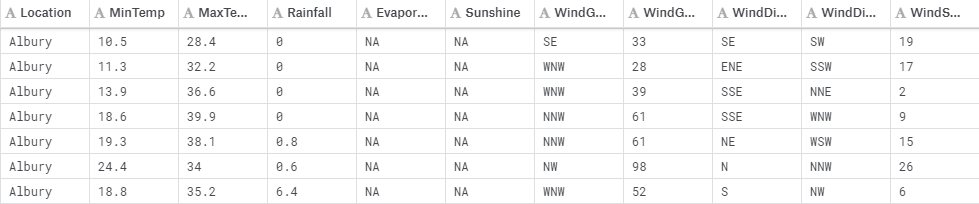
\includegraphics[width=0.85\textwidth]{Pics/data-example.png}
 \caption{Podaci}
 \label{fig:data-example}
\end{figure}

\subsection{Opšti podaci o prognozi}
\label{subsec:opstiPodaci}
Uz pomoć dijagrama će biti predstavljeni neki statistički
podaci atributa.
\begin{itemize}
    \item 
        Predviđanja za kisu tokom merenja su iznosila 22.42\%  za 'Da' i 77.38\% za 'Ne'  (Slika \ref{fig:rainTomorrow}).
    \item 
        Atributi 'Evaporation', 'Sunshine', 'Cloud9am' i 'Cloud3pm' imaju
        43\%, 48\%, 38\%, 40\% nedostajućih vrednosti
\end{itemize}
\begin{figure}[ht]
     \centering
     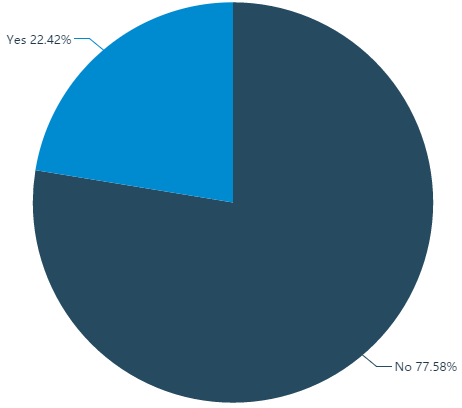
\includegraphics[width=0.5\textwidth]{Pics/rain-tomorrow.png}
     \caption{Atribut RainTomorrow}
     \label{fig:rainTomorrow}
\end{figure}

\subsection{Nedostajuće vrednosti}
\label{subsec:nedostajuceVrednosti}

U samim podacima je bilo nedostajućih vrednosti (Tabela \ref{tab:nans}). Iz prikaza koliko nedostajućih vrednosti ima može se primetiti da je najviše takvih vrednosti bilo u vezi sa atributima gde je trebalo da se koriste speicjalni instrumenti (Evaporation) ili da se vrši merenje bez instrumenata(Cloud9am, Cloud3pm, Sunshine).\par
S obzirom da navedena 4 atributa imaju više od 35\% nedostajućih vrednosti, oni neće učestvovati u daljem istraživanju. Za preostale atribute bilo je jako malo nedostajućih vrednosti, one su obrađene različitim metodama.U programskom jeziku pzthon kategoričke vrednosti su postavljene na vrednosti koje se najviše puta pojavljuju u tom atributu, dok za integer vrednosti je pronađena njihova srednja vrednost i postavljena na nju.\par

\begin{table}[h]
\begin{center}
\caption{Nedostajuće vrednosti}
\label{tab:nans}
\begin{tabular}{|c|c|c|} \hline
\textbf{Atribut} & \textbf{Procenat nedostajućih vrednosti}\\ \hline
Date & 0\% \\ \hline
Location & 0\% \\ \hline
MinTemp & 0\% \\ \hline
MaxTemp & 0\% \\ \hline
Rainfall & 1\% \\ \hline
Evaporation & 43\% \\ \hline
Sunshine & 48\% \\ \hline
WindGustDir & 7\% \\ \hline
WindGustSpeed & 7\% \\ \hline
WindDir9am & 7\% \\ \hline
WindDir3pm & 3\% \\ \hline
WindSpeed9am & 1\% \\ \hline
WindSpeed3pm & 2\% \\ \hline
Humidity9am & 1\% \\ \hline
Humidity3pm & 3\% \\ \hline
Pressure9am & 10\% \\ \hline
Pressure3pm & 10\% \\ \hline
Cloud9am & 38\% \\ \hline
Cloud3pm & 40\% \\ \hline
Temp9am & 1\% \\ \hline
Temp3pm & 2\% \\ \hline
RainToday & 1\% \\ \hline
RainTomorrow & 0\% \\ \hline
\end{tabular}
\end{center}
\end{table}

\subsection{Korelacija među atributima}
\label{subsec:korelacija}
U podacima između atributa postoji veza. Vezu pronalazimo pomoću Pirsonovog koeficijnta korelacije i u nastavku teksta obrađujemo atribute sa koeficijentom većim od 0.8. Kod Drveta odlučivanja parovi atributa u korelaciji nisu izostavljani, dok kod ostalih algoritama, radi njihovog  ubrzanja jedan od parova je isključen. \par
Koeficijent korelacije je računat pomoću IBM SPSS Modeler alata i programskog jezika python. Sledeći kod prikazuje pronalaženje i izbacivanje jednog od atributa sa visokim koeficijentom korelacije.\par
\lstinputlisting[language=Python, caption={Kod za traženje korelacije između atributa},frame=single, label=kod-corel]{Codes/corelation.py}


\subsubsection{Korelacija između 'MinTemp' i 'Temp9am'}
\label{subsubsec:korMinTemp}
Koeficijent korelacije između atributa 'MinTemp' i 'Temp9am' iznsio je 0.901. Vizuelno, korelacija je prikazana na slici \ref{fig:cor-1}. \par
Posmatranjem ova dva atributa, dolazi se do zapažanja da je najniža temperatura u ranim jutarnjim časovima.
\begin{figure}[H]
     \centering
     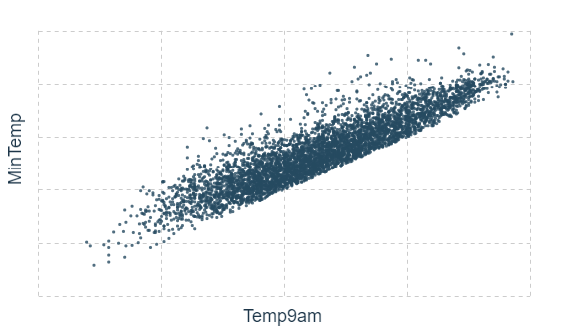
\includegraphics[width=0.8\textwidth]{Pics/corMinTemp.png}
     \caption{'MinTemp' i 'Temp9am'}
     \label{fig:cor-1}
\end{figure}

\subsubsection{Korelacija između 'MaxTemp' i 'Temp3pm'}
\label{subsubsec:korMaxTemp}
Koeficijent korelacija između atributa 'MaxTemp' i 'Temp3pm' iznsio je 0.979. Vizuelno, korelacija je prikazana na slici \ref{fig:cor-2}.\par
Kako je najniža temperatura u ranim jutarnjim satima, iz ove korelacije zapažamo da je dan najtopliji u 15:00 časova.
\begin{figure}[H]
     \centering
     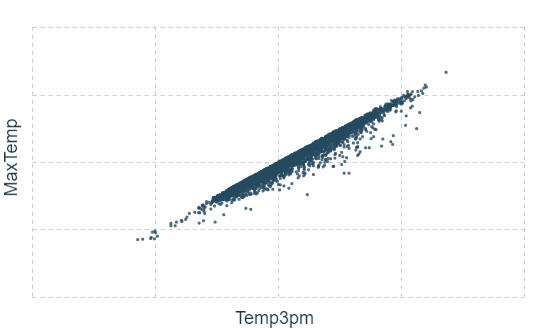
\includegraphics[width=0.8\textwidth]{Pics/corMaxTemp.png}
     \caption{'MaxTemp' i 'Temp3pm'}
     \label{fig:cor-2}
\end{figure}


\subsubsection{Korelacija između 'Pressure9am' i 'Pressure3pm'}
\label{subsubsec:kotP9P3}
Koeficijent korelacija između atributa 'Pressure9am' i 'Pressure3pm' iznsio je 0.957. Vizuelno, korelacija je prikazana na slici \ref{fig:cor-3}\par.
Iz ove korelacije zaključujemo da se pritisak vazduha znatno ne menja izmedjue 9:00 i 15:00.
\begin{figure}[H]
     \centering
     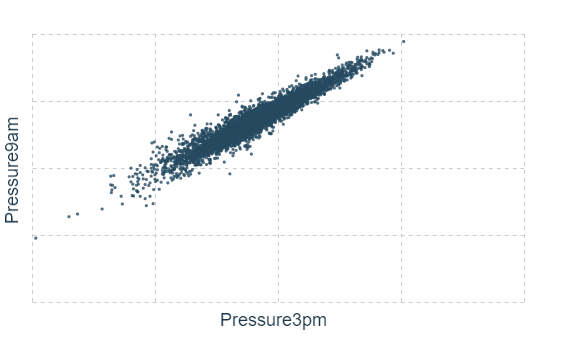
\includegraphics[width=0.8\textwidth]{Pics/corP9P3.png}
     \caption{'Pressure9am' i 'Pressure3pm'}
     \label{fig:cor-3}
\end{figure}


\subsubsection{Korelacija između 'Rainfall' i 'RainToday'}
\label{subsubsec:korRaRT}
Iz zapažanja i iz samog opisa podataka, atribut RainToday zaivisi od Rainfall. Ako je atribut Rainfall > 1.0, RainToday se postavlja na 1 ('Da'), a u drugom slučaju na 0('Ne').\par




\subsection{Predpocesiranje podataka u Python-u}
\label{subsec:predprocess}
Kako algoritmi iz biblioteke scikit-learn\cite{scikit} nemaju automatso predprocesiranje podataka kao IBM SPSS Modeler, predprocesiranje se radi manuelno. Pomoću sledećih kodova se vrši predprocesiranje podataka. 

Učitavanje skupa smo vršili pomoću Pandas \cite{pandas} biblioteke, i čuvali u DataFrame strukturi. Svako pojavljivanje stringa \"NA\" i  praznog stringa  menjamo sa NaN vrednošću iz Nupmhy\cite{numpy} biblioteke np.nan. U slučaju da su se pojavili duplikati u podacima, oni bivaju izbrisani.\par
\lstinputlisting[language=Python, firstline=2, lastline=7, caption = {Učitavanje skupa}]{Codes/python-predprocess.py}


Nedostajuće vrednosti za integer smo menjali sa srednjom vrednošću atributa iz određene kolone, dok smo stringove zamenjivali sa najčešćim stringovima iz date kolone.\par
\lstinputlisting[language=Python, firstline=8, lastline=19, caption = {Uklanjanje NaN vrednosti}]{Codes/python-predprocess.py}

Elemente van granica smo eliminisali iz skupa formula za kvantile, tj ako se element nalazio van $q_1 - 1.5(q_3 - q_1)$ donje granice ili van $q_3 + 1.5(q_3 - q_1)$ gornje granice.
\lstinputlisting[language=Python, firstline=21, lastline=32, caption = {Skidanje elementa van granica}]{Codes/python-predprocess.py}

Kako algoritmi bibliotke sckit-learn rade samo sa numeričkim podacima, vršimo tranformaciju kategoričkih u numeričke preslikavanjem svakog kategoričkog u određen ceo broj.
\lstinputlisting[language=Python, firstline=34, lastline=41, caption = {Transformacija u numeričke}]{Codes/python-predprocess.py}

Vršimo min-max normalizaciju zbog atributa Rainfall koji ima opseg od [0.0 - 250.0].
\lstinputlisting[language=Python, firstline=42, lastline=47, caption = {Normalizacija}]{Codes/python-predprocess.py}

\section{Klasifikacija}
\label{sec:Klasifikacija}
Klasifikacija predstavlja pronalaženje modela koji preslikava skup X u ciljni skup Y ['Da','Ne']. U skupu podataka se javljaju 6 kategoričkih atributa. Predprocesiranjem brišemo elemente van granica iz skupa u python-u, dok u IBM SPSS Modeleru koristimo ugrađene metode.\par

\subsection{Drveta odlučivanja}
\label{sec:DT}
Rezultati koji su se dobijali primenom različitih algoritama su skoro pa ekvivalentni.
Algoritam C\&RT i python su davali nešto lošije rezultate u odnosu na
algoritam C5.0. U IBM SPSS Modeleru i u pythonu smo koristili unakrsnu
validaciju. Skupovi su bili podeljeni na trening(70\%) i test(30\% u pythonu i 20\% u SPSS Modeleru) skupove.\par

\subsubsection{C\&RT}
\label{subsubsec:CART}
U IBM SPSS Modeler-u tok podatakaje izgledao kao na slici \ref{fig:cart-spss}. Nakon učitavanja podataka, pronađeni su elementi van granica i ekstremi, obrađeni su tako što su elementi van granica zamenjeni srednjom vrednošću, a ekstremi pretvoerni u NaN. Nakon toga model je napravljen algoritmom C\&RT.\par Parametri koji su bili podešeni prilikom pravljenja modela su sledeći:
\begin{itemize}
    \item Maximum Tree Depth : 8
    \item Missclassification cost : Actual Yes 2.0
    \item Impurity messure : Gini
\end{itemize}
\par

\begin{figure}[H]
     \centering
     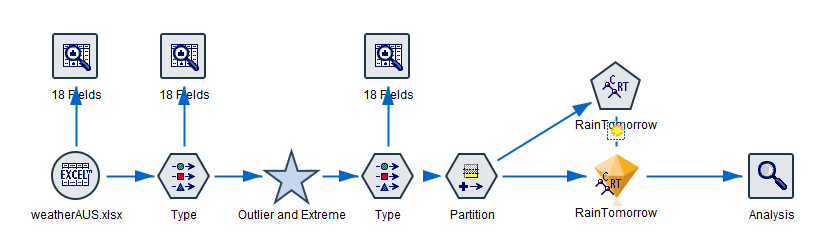
\includegraphics[width=1\textwidth]{Pics/Cart.png}
     \caption{IBM SPSS C\&RT}
     \label{fig:cart-spss}
\end{figure}


Nakon primene skupa podataka na model, dobijaju se sledeći rezultati dati u tabelama \ref{tab:CART-res},  \ref{tab:CART-CM}.
\begin{table}[H]
        \begin{center}
        \caption{Rezultati modela}
        \label{tab:CART-res}
        \begin{tabular}{|c|c|c|c|} \hline
        \textbf{Partition} & \textbf{Training} & \textbf{Testing} &  \textbf{Validation} \\ \hline
        Correct & 81,399 | 81.64\% & 23,089 | 81.69\% & 11,658 | 81.93\% \\ \hline
        Wrong & 18,302 | 18.36\%   & 5,174 | 18.31\% & 2,571 | 18.07\% \\ \hline
        Total & 99,701  & 28,263 & 14,229 \\ \hline
        \end{tabular}
        \end{center}
\end{table}
\begin{table}[H]
        \begin{center}
        \caption{Matrica konfuzije}
        \label{tab:CART-CM}
        \begin{tabular}{|c|c|c|} \hline
        \textbf{} & \textbf{No} & \textbf{Yes} \\ \hline
        No &68,994 & 7,941  \\ \hline
        Yes &  9,805 & 12,388 \\ \hline
        \end{tabular}
        \end{center}
\end{table}
Preciznost modela iznosi oko 82.6\%. Dubina stabla je iznosila 5. Iz rezultata kao i iz podatak se zaključujemo da je instanca  'Ne'  ciljnog atributa dominantnija u odnosu na 'Da'. Iz modela zapažamo da je atribut Humidity3pm jedan od najvažnijih atributa i najviše utiče na određivanje ciljne klase(Slika \ref{fig:cart-importance})\par
\begin{figure}[H]
     \centering
     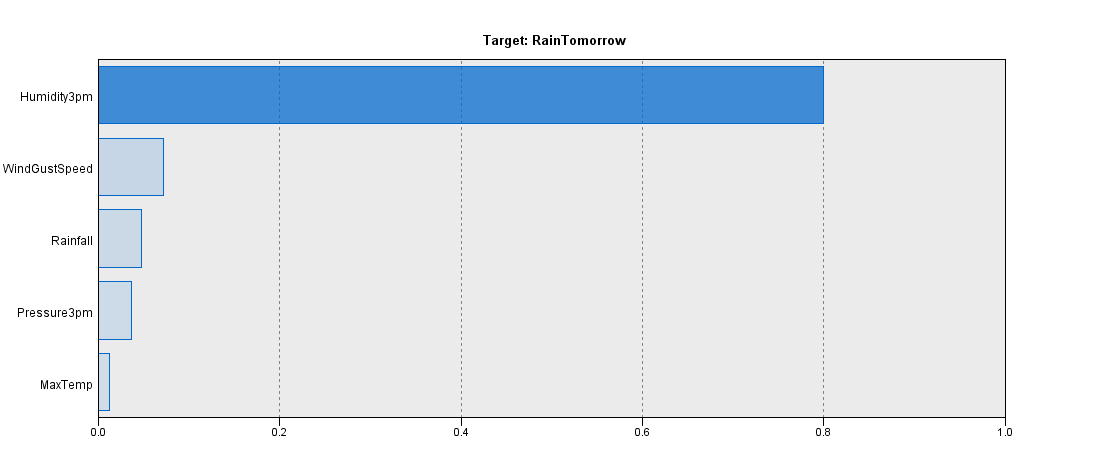
\includegraphics[width=1\textwidth]{Pics/Cart-imporntace.png}
     \caption{Važnost atributa}
     \label{fig:cart-importance}
\end{figure}

\subsubsection{C5.0}
\label{subsubsec:c50}
Tok podataka u IBM SPSS Modeleru je skoro pa identičan kao kod C\&RT obrade. Suštinska razlika je obrada NaN vrednosti za integer tipove i belina za string tipove. Stringovi su obrađenni tako što je nedostajuća vrednost zamenjena sa vrednošću koja se najčešće pojavljuje u podacima za taj atribut sa izuzetkom RainToday gde smo na random način dodeljivali vrednosti. Integer vrednosti su zamenjene uz pomoć C\&RT algoritma.\par

Parametri koji su bili podešeni prilikom pravljenja modela su sledeći:
\begin{itemize}
    \item Cross-Validate : 5
    \item Missclassification cost : Actual Yes 2.0
    \item Favor : Accuracy
\end{itemize}
\par

Nakon primene skupa podataka na model, dobijaju se sledeći rezultati dati u tabelama \ref{tab:C50-res}, \ref{tab:C50-CM}.
\begin{table}[H]
\begin{center}
\caption{Rezultati modela}
\label{tab:C50-res}
\begin{tabular}{|c|c|c|c|} \hline
\textbf{Partition} & \textbf{Training} & \textbf{Testing} &  \textbf{Validation} \\ \hline
Correct & 85,636 | 86.04\% & 24,521 | 82.26\% & 12,221 | 85.86\% \\ \hline
Wrong & 13,893 | 13.96\%   & 3,907 | 13.74\% & 2,021 | 14.14\% \\ \hline
Total & 99,532  & 28,428 & 14,233 \\ \hline
\end{tabular}
\end{center}
\end{table}
\begin{table}[H]
\begin{center}
\caption{Matrica konfuzije nad trening skupom}
\label{tab:C50-CM}
\begin{tabular}{|c|c|c|} \hline
\textbf{} & \textbf{No} & \textbf{Yes} \\ \hline
No &69,675 & 7,443  \\ \hline
Yes &  6,450 & 15,964 \\ \hline
\end{tabular}
\end{center}
\end{table}

Preciznost modela iznosi oko 83\%. Dubina stabla je iznosila 8. C5.0 je precizniji u odnosu na C\&RT zbog poće dubine stable, pa samim tim stablo je komplikovanije (Slika \ref{fig:C50-tree}). Kao i kod C\&RT algoritma atribut sa najvećom važnošću je bio Humidity3pm. 

\begin{figure}[H]
     \centering
     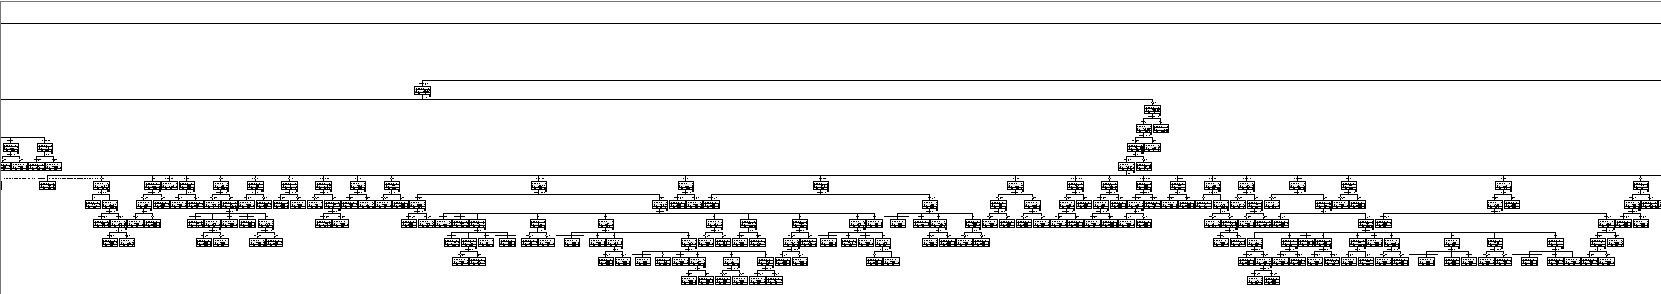
\includegraphics[width=1\textwidth]{Pics/C50-tree.png}
     \caption{Deo stabla C5.0 algoritma}
     \label{fig:C50-tree}
\end{figure}



\subsubsection{Python}
\label{subsubsec:python}
Nakon pretprocesiranja podataka i podele na trening i test skupove, primenom algoritma ( Kod \ref{code:DT} ) dobijaju se sledeći rezultati.
U tabeli \ref{tab:DT-Trening} se nalaze rezultati modela nad trening skupom, a odgovarajuća matrica konfuzije je data u tabeli \ref{tab:DT-Trening-CM}. Nad test skupom rezultati su dati u tabeli \ref{tab:DT-Test} sa odgovarajućom matricom konfuzije u tabeli \ref{tab:DT-Test-CM}.\par
Drveta odlučivanja koja daju približno iste rezultate imaju dubinu stabla između 8 i 10. Iz rezultata zaključujemo da se bolje klasifikuje vrednost atribute 'Ne', što je i očekivano zbog disbalansa atributa RainTomorrow.\par
\newpage
\label{code:DT}
\lstinputlisting[language=python, caption={Drvo odlučivanja},frame=single, label=kod-dt]{Codes/DT.py}

\begin{itemize}
    \item Trening Skup\\
        Preciznost nad celim trening skupom je iznsila oko 89.56\% (0.8956)
        % \restylefloat{table}
        \begin{table}[H]
        \begin{center}
        \caption{Rezultati nad trening skupom}
        \label{tab:DT-Trening}
        \begin{tabular}{|c|c|c|c|c|} \hline
        \textbf{Class} & \textbf{precision} & \textbf{recall}  & \textbf{f1-score} & \textbf{support} \\ \hline
        Yes & 0.61   &   0.34  &    0.43 &     5004 \\ \hline
         No & 0.90   &   0.98  &    0.94   &  63633\\ \hline
        \end{tabular}
        \end{center}
        \end{table}
        
        \begin{table}[H]
        \begin{center}
        \caption{Matrica konfuzije}
        \label{tab:DT-Trening-CM}
        \begin{tabular}{|c|c|c|} \hline
        \textbf{} & \textbf{Yes} & \textbf{No} \\ \hline
        Yes & 4552 & 6804  \\ \hline
        No &  1223 &61609 \\ \hline
        \end{tabular}
        \end{center}
        \end{table}
        
    \item Test Skup\\
        Preciznost nad celim test skupom je iznsila oko 86.29\% (0.8629) 
    \begin{table}[H]
        \begin{center}
        \caption{Rezultati nad test skupom}
        \label{tab:DT-Test}
        \begin{tabular}{|c|c|c|c|c|} \hline
        \textbf{Class} & \textbf{precision} & \textbf{recall}  & \textbf{f1-score} & \textbf{support} \\ \hline
        No & 0.89   &   0.96  &    0.92    & 27237\\ \hline
        Yes &  0.61  &    0.34   &   0.43    &  5004\\ \hline
        \end{tabular}
        \end{center}
    \end{table}
    \begin{table}[H]
        \begin{center}
        \caption{Matrica konfuzije}
        \label{tab:DT-Test-CM}
        \begin{tabular}{|c|c|c|} \hline
        \textbf{} & \textbf{Yes} & \textbf{No} \\ \hline
        Yes &1498  &3369  \\ \hline
        No &  3942 &25986 \\ \hline
        \end{tabular}
        \end{center}
    \end{table}
\end{itemize}




\subsection{Metod potpornih vektora}
\label{SVM}
Pravljenje modela metodom potpornih vektora je dosta procesorski zahtevnije od drveta odlučivanja pa će mo vaditi uzorak skupa i praviti model nad njim. Izdvojen je uzorak veličine 30\%, takođe je smanjena dimenzionalnost pomoću prethodno izračunatih korelacija. Pored korelacija je korišćen metod PCA za smanjenje dimenzionalnosti.\par
Nedostajuće vrednosti su zamenjene odgovarajućim pomoću C\&RT algoritma, dok su ekstremi odbačeni a elementi van granica zamenjeni srednjom vrednošću odgovarajućih atributa. Za prvaljenje modela je izabran polinomjalni kernel sa parametrom C koji iznosi 8.

\begin{figure}[H]
     \centering
     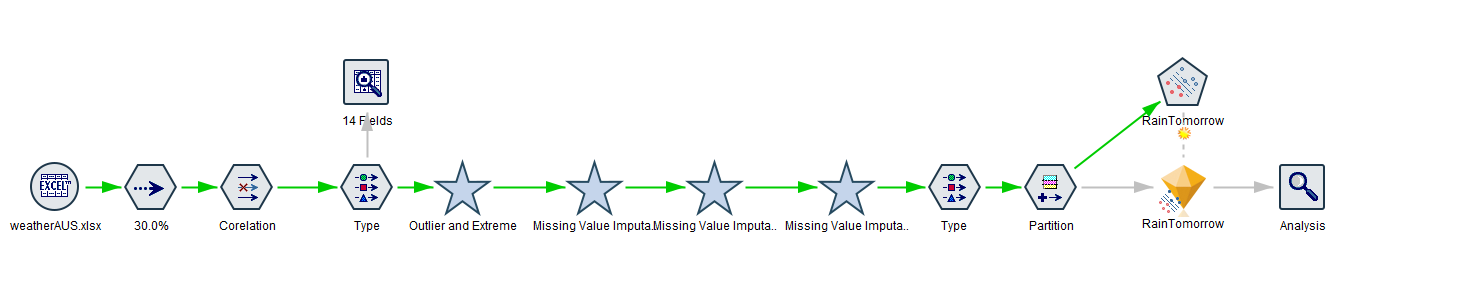
\includegraphics[width=1\textwidth]{Pics/SVM.png}
     \caption{IBM SPSS SVM}
     \label{fig:svm-spss}
\end{figure}
Rezultati koji se dobijaju su u tabeli \ref{tab:SVM-res} sa odgovarajućom matricom konfuzije nad trening skupom \ref{tab:SVM-CM-train} i nad test skupom \ref{tab:SVM-CM-test}. Preciznost modela je iznosila 83.37\% nad smanjenom skupu, a nad originalnom 70.42\%. Iz rezultata zaključujemo da se instanca 'Ne' atributa RainTomorrow bojle klasifikuje od instance 'Da' što oslikava manjinu instanci 'Da' u orginalnom skupu.


\begin{table}[H]
        \begin{center}
        \caption{Rezultati modela}
        \label{tab:SVM-res}
        \begin{tabular}{|c|c|c|} \hline
        \textbf{Partition} & \textbf{Training} & \textbf{Testing}\\ \hline
        Correct & 20,943 | 83.32 \% & 9,070 | 83.42 \% \\ \hline
        Wrong    & 4,193 | 16.68 \% & 1,803 | 16.58 \% \\ \hline
        Total & 25,163  & 10,873 \\ \hline
        \end{tabular}
        \end{center}
\end{table}

\begin{table}[H]
        \begin{center}
        \caption{Matrica konfuzije nad tretning skupom}
        \label{tab:SVM-CM-train}
        \begin{tabular}{|c|c|c|} \hline
        \textbf{} & \textbf{No} & \textbf{Yes} \\ \hline
        No & 17,268 & 2,310  \\ \hline
        Yes & 1,883 & 3,675 \\ \hline
        \end{tabular}
        \end{center}
\end{table}
\begin{table}[H]
        \begin{center}
        \caption{Matrica konfuzije nad test skupom}
        \label{tab:SVM-CM-test}
        \begin{tabular}{|c|c|c|} \hline
        \textbf{} & \textbf{No} & \textbf{Yes} \\ \hline
        No & 7,458 & 991  \\ \hline
        Yes &  812 & 1,612 \\ \hline
        \end{tabular}
        \end{center}
\end{table}
% 23 min obican
%  7min
Prilikom korišćenja metoda PCA za smanjenje dimenzionalnosti, dobija se ubrazanje od 330\%. Izabranih 6 atributa objašnjavaju 96.5\% skupa. (Slika \ref{fig:svm-pca}). \par
Rezultati modela se nalaze u tabeli \ref{tab:PCA-res}. Postignuta preciznost iznosi 84.21\%. Zaključujemo da primenom PCA tehnike smanjenja dimenzionalnostii znatno se ubrzavamo pronalaženje ciljnog atributa, ali sa cenom da gubimo neke informacije u podacima.

\begin{figure}[H]
     \centering
     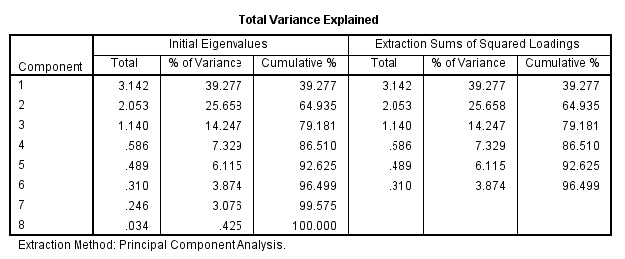
\includegraphics[width=1\textwidth]{Pics/svm-pca.png}
     \caption{PCA}
     \label{fig:svm-pca}
\end{figure}

\begin{table}[H]
        \begin{center}
        \caption{Rezultati modela}
        \label{tab:PCA-res}
        \begin{tabular}{|c|c|c|} \hline
        \textbf{Partition} & \textbf{Training} & \textbf{Testing}\\ \hline
        Correct & 21,651 | 84.14 \% & 9,090 | 84.28 \% \\ \hline
        Wrong    & 4,081 | 15.86 \% & 1,696 | 15.72 \% \\ \hline
        Total & 25,163  & 10,873 \\ \hline
        \end{tabular}
        \end{center}
\end{table}

U programskom jeziku python, tražili smo najbolje parametre za model pomoću uzoračkog skupa.. Uzorački skup je sadržao 20\% originalnog skupa,

\label{code:SVM}
\lstinputlisting[language=python, caption={SVM parametri},frame=single, label=kod-svm]{Codes/SVM.py}

Rezultati koje dobijamo nakon izvršavanja koda su:
\begin{itemize}
    \item C : 5
    \item coef0 : 0.5
    \item degree : 3
    \item gamma : 1
    \item kernel : poly
\end{itemize}

Preciznost nad trening skupom je iznosila 87.7\% sa propratnim rezultatima datim u tabeli \ref{tab:SVM-py-train}, a nad test skupom preciznost je iznosila 87.2\% sa rezultatima datim u tabeli \ref{tab:SVM-py-test}. Matrica konfuzije nad trening skupom data je u tabeli \ref{tab:SVM-trening-CM} i nad test skupom u tabeli \ref{tab:SVM-test-CM}.\par
Iz rezultata možemo zaključiti da je uzorak sadržao veći broj instanci 'Ne', i samim tim prave instance 'Da' lošije klasifikovano, tačnije klasifikovane su kao 'Ne'.
% \restylefloat{table}
    \begin{table}[H]
        \begin{center}
        \caption{Rezultati nad trening skupom}
        \label{tab:SVM-py-train}
        \begin{tabular}{|c|c|c|c|c|} \hline
        \textbf{Class} & \textbf{precision} & \textbf{recall}  & \textbf{f1-score} & \textbf{support} \\ \hline
        Yes & 0.80    &  0.26    &  0.39    &  2225 \\ \hline
        No & 0.88  &    0.99    &  0.93 & 12465\\ \hline
        \end{tabular}
        \end{center}
    \end{table}
        
    \begin{table}[H]
        \begin{center}
        \caption{Rezultati nad test skupom}
        \label{tab:SVM-py-test}
        \begin{tabular}{|c|c|c|c|c|} \hline
        \textbf{Class} & \textbf{precision} & \textbf{recall}  & \textbf{f1-score} & \textbf{support} \\ \hline
        Yes &  0.77  &    0.23  &    0.35  &     954 \\ \hline
        No & 0.88  &    0.99  &    0.93  &    5342 \\ \hline
        \end{tabular}
        \end{center}
    \end{table}
    
        \begin{table}[H]
        \begin{center}
        \caption{Matrica konfuzije trening skupa}
        \label{tab:SVM-trening-CM}
        \begin{tabular}{|c|c|c|} \hline
        \textbf{} & \textbf{Yes} & \textbf{No} \\ \hline
        Yes & 568 & 1657  \\ \hline
        No & 140 & 12325 \\ \hline
        \end{tabular}
        \end{center}
        \end{table}
        
        \begin{table}[H]
        \begin{center}
        \caption{Matrica konfuzije test skupa}
        \label{tab:SVM-test-CM}
        \begin{tabular}{|c|c|c|} \hline
        \textbf{} & \textbf{Yes} & \textbf{No} \\ \hline
        Yes & 217 &  737  \\ \hline
        No & 66 & 5276 \\ \hline
        \end{tabular}
        \end{center}
        \end{table}
        



\subsection{K-najbližih suseda}
\label{KNN}
Kod algoritma K najbližih suseda kao kod metoda potpornih vektora, smanjujemo dimenzionalnost skupa prethodno izračunatom korelacijom, pravimo uzorački skup koji sadrži 30\% originalnog skupa, ekstremne vrednosti brišemo i elemente van granica postavljamo na srednje vrednosti. Nedostajuće vrednosti zamenjujemo vrednostima izračunatim pomoć C\&RT algoritma.\par
Prilikom pravljenja modela postavljamo broj suseda na 3 (K=3), a za distancu euklidsko rastojanje. Model je prikazan na slici \ref{fig:knn-graph}.

\begin{figure}[H]
     \centering
     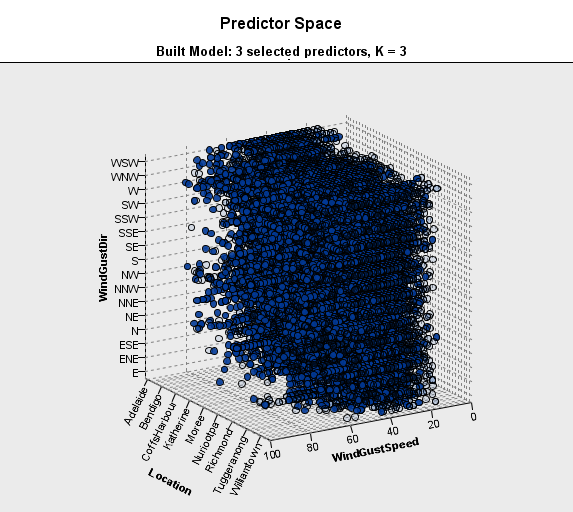
\includegraphics[width=0.8\textwidth]{Pics/KNN-grap.png}
     \caption{KNN Model}
     \label{fig:knn-graph}
\end{figure}

Kao rezultat izvršavanja modela nad podacima dobijaju se sledeći rezultati prikazani u narednim tabelama. Rezultat modela je dat u tabeli \ref{tab:KNN-res} i matrice konfuzije nad trening skupom \ref{tab:KNN-training-CM} i nad test skupom \ref{tab:KNN-testing-CM}. Ukupna preciznost modela za uzorak je iznosila 81.94\%\par


\begin{table}[H]
        \begin{center}
        \caption{Rezultati modela}
        \label{tab:KNN-res}
        \begin{tabular}{|c|c|c|} \hline
        \textbf{Partition} & \textbf{Training} & \textbf{Testing}\\ \hline
        Correct & 20,722 | 82.03 \% & 8,840 | 81.85 \% \\ \hline
        Wrong    & 4,539 | 17.97 \% & 1,960 | 18.15 \% \\ \hline
        Total & 25,261  & 10,800 \\ \hline
        \end{tabular}
        \end{center}
\end{table}
\begin{table}[H]
        \begin{center}
        \caption{Matrica konfuzije tretning skupa}
        \label{tab:KNN-training-CM}
        \begin{tabular}{|c|c|c|} \hline
        \textbf{} & \textbf{No} & \textbf{Yes} \\ \hline
        No & 18,367 & 1,339  \\ \hline
        Yes & 3,200 & 2,355 \\ \hline
        \end{tabular}
        \end{center}
\end{table}

\begin{table}[H]
        \begin{center}
        \caption{Matrica konfuzije test skupa}
        \label{tab:KNN-testing-CM}
        \begin{tabular}{|c|c|c|} \hline
        \textbf{} & \textbf{No} & \textbf{Yes} \\ \hline
        No & 7,836 & 531  \\ \hline
        Yes &  1,429 & 1,004 \\ \hline
        \end{tabular}
        \end{center}
\end{table}

Iz matrica kofnuzije, kao i u prethodnim algoritmima, 'Da' kao ciljni atribut  se lošije klasifikuje od 'Ne', zbog neizbalansiranosti ciljnog atributa.

U programskom jeziku python, tražili smo najbolje parametre nad našim skupom prilikom pravljenja modela. Skup je bio uzorak od 30\% originalnog skupa.
Kao rezultat izvršavanja koda \ref{code:KNN}, dobijaju se sledeći paramteri:
\begin{itemize}
    \item n\_neighbors = 4
    \item p = 2
    \item  weights = 'uniform'
\end{itemize}

\label{code:KNN}
\lstinputlisting[language=python, caption={KNN parametri},frame=single, label=kod-knn]{Codes/KNN.py}

Rezultati koji se dobijaju su dati u sledećim tabelama. Iz samih rezultata možemo da primetimo da je došlo do malog predprilagođavanja podataka, tj. nad trening skupom preciznost modela je iznosila 90\% dok je nad test skupom iznosila 83\%.\par




Možemo da primetimo da se 'Da' malo lošije klasifikuje od 'Ne' u trening skupu, dok se u test skupu preciznost 'Da' drastično smanjila, tačnije iznosi 47\%. To se može i videti iz matrica konfuzija.\par
    \begin{table}[H]
        \begin{center}
        \caption{Rezultati nad trening skupom}
        \label{tab:KNN-py-train}
        \begin{tabular}{|c|c|c|c|c|} \hline
        \textbf{Class} & \textbf{precision} & \textbf{recall}  & \textbf{f1-score} & \textbf{support} \\ \hline
        Yes &  0.70&      0.60  &    0.65   &   3408 \\ \hline
        No & 0.93    &  0.95 &     0.94   &  18665 \\ \hline
        \end{tabular}
        \end{center}
    \end{table}
        
    \begin{table}[H]
        \begin{center}
        \caption{Rezultati nad test skupom}
        \label{tab:KNN-py-test}
        \begin{tabular}{|c|c|c|c|c|} \hline
        \textbf{Class} & \textbf{precision} & \textbf{recall}  & \textbf{f1-score} & \textbf{support} \\ \hline
        Yes &  0.47    &  0.37     & 0.41  &    1461 \\ \hline
        No & 0.89   &   0.92   &  0.91    &  8000 \\ \hline
        \end{tabular}
        \end{center}
    \end{table}
    
        \begin{table}[H]
        \begin{center}
        \caption{Matrica konfuzije trening skupa}
        \label{tab:KNN-py-train-CM}
        \begin{tabular}{|c|c|c|} \hline
        \textbf{} & \textbf{Yes} & \textbf{No} \\ \hline
        Yes & 2048  &1360  \\ \hline
        No & 888  &17777 \\ \hline
        \end{tabular}
        \end{center}
        \end{table}
        
        \begin{table}[H]
        \begin{center}
        \caption{Matrica konfuzije test skupa}
        \label{tab:KNN-py-test-CM}
        \begin{tabular}{|c|c|c|} \hline
        \textbf{} & \textbf{Yes} & \textbf{No} \\ \hline
        Yes & 539 & 922 \\ \hline
        No & 618 & 7382 \\ \hline
        \end{tabular}
        \end{center}
        \end{table}
        

\subsection{Veštačke neuronkse mreže}
\label{NN}
Za pravljenje modela neuronskih mreža, dimenzionalnost podataka smanjujemo prethodno izračunatim korelacijama, nedostajuće vrednosti računamo i dopunjujemo pomoću C\&RT algoritma, elemente van granica zamenjujemo odgovarajućim srednjim vrednostima i ekstremne vrednosti nuliramo.

Kao rezultat dobijamo model prikazan na slici \ref{fig:NN-graph} i odgovarajuće vrednosti date u tabeli \ref{tab:NN-res}. Neuronske mreže imaju 1 skriveni sloj. Koristimo RBF model za neuronske mreže. Najvažniji atribut je Humidity3pm (Slika \ref{fig:NN-importance}).

\begin{figure}[H]
     \centering
     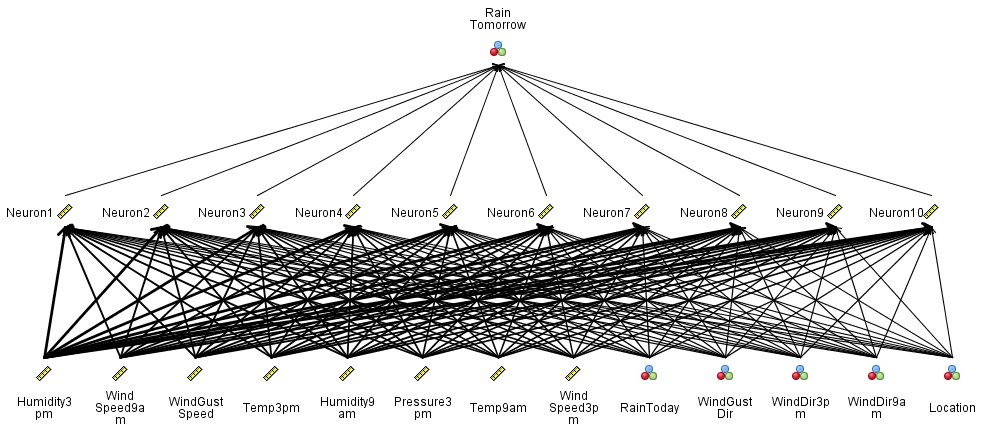
\includegraphics[width=1\textwidth]{Pics/NN-graph.png}
     \caption{Neuronske mreže}
     \label{fig:NN-graph}
\end{figure}

\begin{figure}[H]
     \centering
     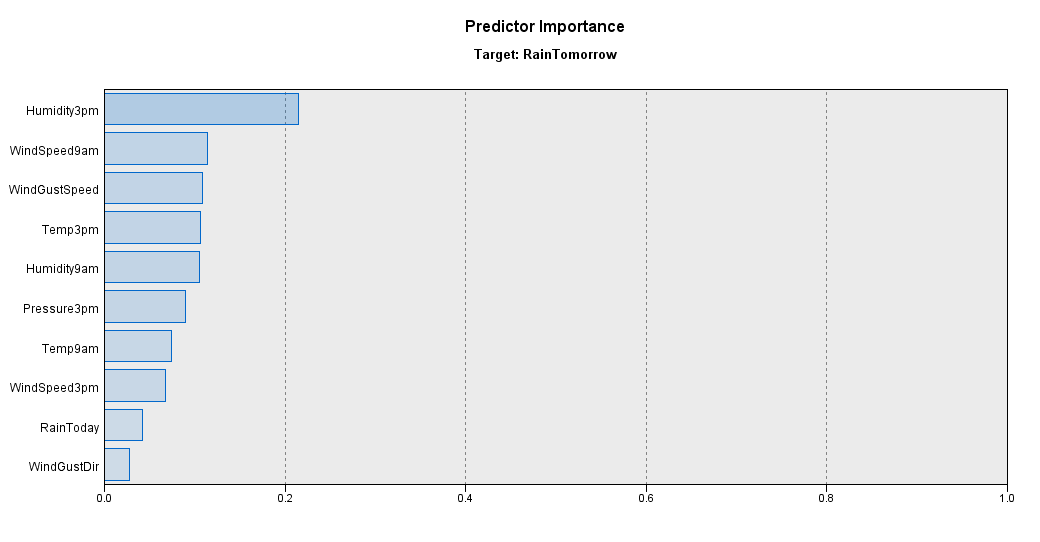
\includegraphics[width=1\textwidth]{Pics/NN-importance.png}
     \caption{Važnost atributa}
     \label{fig:NN-importance}
\end{figure}

\begin{table}[H]
        \begin{center}
        \caption{Rezultati modela}
        \label{tab:NN-res}
        \begin{tabular}{|c|c|c|} \hline
        \textbf{Partition} & \textbf{Training} & \textbf{Testing}\\ \hline
        Correct & 69,447 | 82.5 \% & 30,097 | 82.64 \% \\ \hline
        Wrong   & 14,734 | 17.5 \% & 6,322  | 17.36 \% \\ \hline
        Total & 84,181  & 36,419 \\ \hline
        \end{tabular}
        \end{center}
\end{table}

\begin{table}[H]
        \begin{center}
        \caption{Matrica konfuzije nad tretning skupom}
        \label{tab:NN-CM-train}
        \begin{tabular}{|c|c|c|} \hline
        \textbf{} & \textbf{No} & \textbf{Yes} \\ \hline
        No & 62,751 & 2,734  \\ \hline
        Yes & 12,000 & 6,696 \\ \hline
        \end{tabular}
        \end{center}
\end{table}
\begin{table}[H]
        \begin{center}
        \caption{Matrica konfuzije nad test skupom}
        \label{tab:NN-CM-test}
        \begin{tabular}{|c|c|c|} \hline
        \textbf{} & \textbf{No} & \textbf{Yes} \\ \hline
        No & 27,231 & 1,206  \\ \hline
        Yes &  5,116 & 2,866 \\ \hline
        \end{tabular}
        \end{center}
\end{table}

Preciznost modela je iznosila 82.57 \%, sa tim da se instanca 'Da' atributa RainTomorrow skoro duplo više klasifikuje kao 'Ne', to se može videti i iz matrica konfuzije (Tabele \ref{tab:NN-CM-train} i \ref{tab:NN-CM-test}). \par

U radu sa mrežama u pythonu, postavljamo sledeće paramtre i trazimo najbolji paramtar. Za testiranje ovih parametara uzimamo uzorak od 20\% iz originalnog skupa. Kao rezultat se dobija:
\begin{itemize}
    \item solver : adam
    \item activation : relu 
    \item learning\_rate : adaptive
\end{itemize}
\label{code:NN}
\lstinputlisting[language=python, caption={NN parametri},frame=single, label=kod-nn]{Codes/NN.py}

Nakon pronalaženja najboljih paramtetara, treniramo model nad celim skupom. Rezultat je prikazan u sledećoj tabeli za trening skup \ref{tab:NN-py-train} sa matricom konfuzije \ref{tab:NN-trening-CM} i za test skup \ref{tab:NN-py-test} sa matricom konfuzije \ref{tab:NN-test-CM}.\par


\begin{table}[H]
        \begin{center}
        \caption{Rezultati nad trening skupom}
        \label{tab:NN-py-train}
        \begin{tabular}{|c|c|c|c|c|} \hline
        \textbf{Class} & \textbf{precision} & \textbf{recall}  & \textbf{f1-score} & \textbf{support} \\ \hline
        Yes &  0.70&      0.29    &  0.41   &  11356 \\ \hline
        No & 0.88   &   0.98   &   0.93  &   62832 \\ \hline
        \end{tabular}
        \end{center}
    \end{table}
        
    \begin{table}[H]
        \begin{center}
        \caption{Rezultati nad test skupom}
        \label{tab:NN-py-test}
        \begin{tabular}{|c|c|c|c|c|} \hline
        \textbf{Class} & \textbf{precision} & \textbf{recall}  & \textbf{f1-score} & \textbf{support} \\ \hline
        Yes &  0.70   &   0.28   &   0.40    &  4867 \\ \hline
        No & 0.88   &   0.98   &   0.93   &  26928 \\ \hline
        \end{tabular}
        \end{center}
    \end{table}
    
        \begin{table}[H]
        \begin{center}
        \caption{Matrica konfuzije trening skupa}
        \label{tab:NN-trening-CM}
        \begin{tabular}{|c|c|c|} \hline
        \textbf{} & \textbf{Yes} & \textbf{No} \\ \hline
        Yes &  3251&  8105  \\ \hline
        No &  1399 &61433 \\ \hline
        \end{tabular}
        \end{center}
        \end{table}
        
        \begin{table}[H]
        \begin{center}
        \caption{Matrica konfuzije test skupa}
        \label{tab:NN-test-CM}
        \begin{tabular}{|c|c|c|} \hline
        \textbf{} & \textbf{Yes} & \textbf{No} \\ \hline
        Yes & 1385 & 3482  \\ \hline
        No & 592 & 26336 \\ \hline
        \end{tabular}
        \end{center}
        \end{table}

\newpage
\section{Zaključak}
\label{sec:zakljucak}

Primenom algoritama klasifikacije dobija se približno ista preciznost modela različitih algoritama. Međutim neki algoritmi daju bolje rezultate od drugih, neki bolje klasifiku instancu 'Da', a neki su dosta brži prilikom pravljenja modela. Algoritam koji je najbolje klasifikovao instacu 'Da' je bio C5.0 sa preciznošću od 83\%, dok algoritam za drveta odlučivanja u pythonu je imao najveću preciznost od 87\%.\par
Ono što možemo da zaključimo svaki algoritam je davao prilično dobre rezultate sa malim odstupanjima, bilo koji metod da se izabere, na kraju će model dobro klasifikovati ciljnu klasu, tačnije predviđanje o sutrašnjoj prognozi.

% \appendix
% \section{Dodatak}
% % Ovde pišem dodatne stvari, ukoliko za time ima potrebe.
% % Ovde pišem dodatne stvari, ukoliko za time ima potrebe.
% % Ovde pišem dodatne stvari, ukoliko za time ima potrebe.
% % Ovde pišem dodatne stvari, ukoliko za time ima potrebe.
% % Ovde pišem dodatne stvari, ukoliko za time ima potrebe.

\newpage
\addcontentsline{toc}{section}{Literatura}
\appendix
\bibliography{seminarski} 
\bibliographystyle{plain}

\end{document}
